\documentclass[12pt,spanish,a5paper,landscape]{article}
\usepackage[utf8]{inputenc}
\usepackage{babel}
\usepackage{listings}
\usepackage{mathpazo}
\usepackage{courier}
\usepackage{xcolor}
\usepackage{textcomp}
\usepackage{amsmath}
\usepackage{amssymb}
\usepackage{tikz}
\usepackage{geometry}

\newcommand{\onelinerule}{\rule[2.3ex]{0pt}{0pt}}
\newcommand{\twolinerule}{\rule[6.2ex]{0pt}{0pt}}
\newcommand{\respuesta}{\framebox[\textwidth]{\twolinerule}}
\newcommand{\nombre}{%
  \begin{tikzpicture}[xscale=.4,yscale=.7]
    \draw (0, 0) rectangle (22, 1);
  \end{tikzpicture}%
}
%\newcommand{\rol}   {\framebox[0.3\textwidth]{\onelinerule}}
\newcommand{\rol}{%
  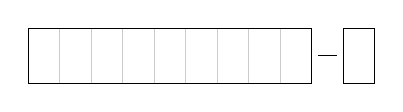
\begin{tikzpicture}[xscale=.4,yscale=.7]
    \draw[gray!40] ( 0, 0) grid      ( 9, 1);
    \draw          ( 0, 0) rectangle ( 9, 1);
    \draw          (10, 0) rectangle (11, 1);
    \draw (9 + .2, .5) -- (10 - .2, .5);
  \end{tikzpicture}%
}
\newcommand{\li}{\lstinline}
\providecommand{\pond}[1]{[{\small\textbf{#1\%}}]}

\lstdefinelanguage{py}{%
  classoffset=0,%
    morekeywords={%
      False,class,finally,is,return,None,continue,for,lambda,try,%
      True,def,from,nonlocal,while,and,del,global,not,with,print,%
      as,elif,if,or,yield,assert,else,import,pass,break,except,in,raise},%
    keywordstyle=\color{black!80}\bfseries,%
  classoffset=1,
    morekeywords={int,float,str,abs,len,raw_input,exit,range,min,max,%
      set,dict,tuple,list,bool,complex,round,sum,all,any,zip,map,filter,%
      sorted,reversed,dir,file,frozenset,open,%
      array,zeros,ones,arange,linspace,eye,diag,dot},
    keywordstyle=\color{black!50}\bfseries,%
  classoffset=0,%
  sensitive=true,%
  morecomment=[l]\#,%
  morestring=[b]',%
  morestring=[b]",%
  stringstyle=\em,%
}

\lstdefinelanguage{testcase}{%
  moredelim=[is][\bfseries]{`}{`},%
  backgroundcolor=\color{gray!20},%
}

\lstdefinelanguage{file}{%
  frame=single,%
}

\lstset{language=py}
\lstset{basicstyle=\ttfamily}
\lstset{columns=fixed}
\lstset{upquote=true}
\lstset{showstringspaces=false}
\lstset{rangeprefix=\#\ }
\lstset{includerangemarker=false}

\newlist{certamen}{enumerate}{1}
\setlist[certamen]{%
  label=\arabic*.,
  font=\LARGE\bfseries,%
  labelindent=-.5in,%
  leftmargin=0pt,%
  labelsep=1em%
}


\lstset{frame=single}
\lstset{language=testcase}

\parskip 1ex
\parindent 0pt

\begin{document}
  \pagestyle{empty}
  \thispagestyle{empty}

  \part*{Control 1, miércoles 1--2}
  \newpage

  En un juego de naipes entre dos jugadores,
  cada uno de ellos recibe dos cartas numeradas del 1 al 13.
  Cuando las dos cartas de un jugador tienen el mismo número,
  decimos que él tiene una \emph{pareja}.
  El juego lo gana el jugador que tiene una pareja.

  Por supuesto,
  podría ocurrir que ambos tienen una pareja.
  En este caso hay un empate.

  Cuando ninguno tiene una pareja,
  gana el que tiene las cartas más cercanas entre ellas.
  Si están igual de cercanas, es un empate.

  Escriba un programa que pregunte las cartas,
  y diga quién ganó.
  Su programa debe verse como los de los ejemplos.

  \begin{minipage}{0.25\textwidth}
    \lstinputlisting%
      [linerange=CASO\ 1-FIN\ CASO\ 1]%
      {casos-miercoles-1-2.txt}
  \end{minipage}
  \hspace{1em}
  \begin{minipage}{0.25\textwidth}
    \lstinputlisting%
      [linerange=CASO\ 2-FIN\ CASO\ 2]%
      {casos-miercoles-1-2.txt}
  \end{minipage}
  \hspace{1em}
  \begin{minipage}{0.25\textwidth}
    \lstinputlisting%
      [linerange=CASO\ 3-FIN\ CASO\ 3]%
      {casos-miercoles-1-2.txt}
  \end{minipage}

  \newpage
  \part*{Control 1, miércoles 3--4}
  \newpage

  En un juego de naipes entre dos jugadores,
  cada uno de ellos recibe dos cartas numeradas del 1 al 13.
  Cuando las dos cartas de un jugador son consecutivas
  (por ejemplo un 5 y un 6)
  decimos que él tiene una \emph{escalera}.
  El juego lo gana el jugador que tiene una escalera.

  Por supuesto,
  podría ocurrir que ambos tienen una escalera.
  En este caso hay un empate.

  Cuando ninguno tiene una escalera,
  gana el que tiene la carta menor.
  Si ambos tienen la misma carta menor, es un empate.

  Escriba un programa que pregunte las cartas,
  y diga quién ganó.
  Su programa debe verse como los de los ejemplos.

  \begin{minipage}{0.25\textwidth}
    \lstinputlisting%
      [linerange=CASO\ 1-FIN\ CASO\ 1]%
      {casos-miercoles-3-4.txt}
  \end{minipage}
  \hspace{1em}
  \begin{minipage}{0.25\textwidth}
    \lstinputlisting%
      [linerange=CASO\ 2-FIN\ CASO\ 2]%
      {casos-miercoles-3-4.txt}
  \end{minipage}
  \hspace{1em}
  \begin{minipage}{0.25\textwidth}
    \lstinputlisting%
      [linerange=CASO\ 3-FIN\ CASO\ 3]%
      {casos-miercoles-3-4.txt}
  \end{minipage}

  \newpage
  \part*{Control 1, jueves 1--2}
  \newpage

  En un juego de naipes entre dos jugadoras,
  cada una de ellas recibe dos cartas.
  Cada carta puede ser
  pica (\verb+p+),
  corazón (\verb+c+),
  trébol (\verb+t+) o
  diamante (\verb+d+).
  El juego lo gana la jugadora que tiene dos cartas iguales.

  Por supuesto,
  podría ocurrir que ambas tengan cartas iguales,
  o que ninguna de ellas las tengan.
  Cuando esto ocurre, gana la que tenga algun corazón.
  Si este criterio no es suficiente para determinar a la ganadora,
  es un empate.

  Escriba un programa que pregunte las cartas,
  y diga quién ganó.
  Su programa debe verse como los de los ejemplos.

  \begin{minipage}{0.25\textwidth}
    \lstinputlisting%
      [linerange=CASO\ 1-FIN\ CASO\ 1]%
      {casos-jueves-1-2.txt}
  \end{minipage}
  \hspace{1em}
  \begin{minipage}{0.25\textwidth}
    \lstinputlisting%
      [linerange=CASO\ 2-FIN\ CASO\ 2]%
      {casos-jueves-1-2.txt}
  \end{minipage}
  \hspace{1em}
  \begin{minipage}{0.25\textwidth}
    \lstinputlisting%
      [linerange=CASO\ 3-FIN\ CASO\ 3]%
      {casos-jueves-1-2.txt}
  \end{minipage}

  \newpage
  \part*{Control 1, jueves 3--4}
  \newpage

  En un juego de naipes entre dos jugadoras,
  cada una de ellas recibe dos cartas.
  Cada carta puede ser
  pica (\verb+p+),
  corazón (\verb+c+),
  trébol (\verb+t+) o
  diamante (\verb+d+).

  El juego lo gana la jugadora que tenga más tréboles.
  Si ambas tienen la misma cantidad de tréboles,
  es un empate.

  Escriba un programa que pregunte las cartas,
  y diga quién ganó.
  Su programa debe verse como los de los ejemplos.

  \begin{minipage}{0.25\textwidth}
    \lstinputlisting%
      [linerange=CASO\ 1-FIN\ CASO\ 1]%
      {casos-jueves-3-4.txt}
  \end{minipage}
  \hspace{1em}
  \begin{minipage}{0.25\textwidth}
    \lstinputlisting%
      [linerange=CASO\ 2-FIN\ CASO\ 2]%
      {casos-jueves-3-4.txt}
  \end{minipage}
  \hspace{1em}
  \begin{minipage}{0.25\textwidth}
    \lstinputlisting%
      [linerange=CASO\ 3-FIN\ CASO\ 3]%
      {casos-jueves-3-4.txt}
  \end{minipage}

\end{document}

